\documentclass[11pt]{article}

%\usepackage[brazilian]{babel}
\usepackage[utf8]{inputenc}
\usepackage[T1]{fontenc}
\usepackage{lmodern}
\usepackage{amsmath,amsfonts}
\usepackage{subfigure}
\usepackage{bm}
\usepackage{listings}
\usepackage{pifont}%
\usepackage{xcolor}
\usepackage{siunitx}

\usepackage{pgfplots,tikz}
\usepackage{fullpage}      % Margens
\usepackage{indentfirst}   % Autoidentar
\usepackage{graphicx}       % Pictures

\newcommand{\answer}[1]{\color{blue}{#1}\color{black}}
\sisetup{scientific-notation = engineering}%

\begin{document}

\noindent\answer{Gerald LaMountain}

\noindent Northeastern University
\hfill April 10, 2018

\noindent Department of Electrical and Computer Engineering
\hfill EECE5698-ST (Spring 2018)

\noindent {} \hfill \textbf{Homework 4}

\noindent \rule{\linewidth}{1.5pt}

\vspace*{.5cm}

\underline{Due date}: Friday 20, April 2018. Hand in at class or send a scanned copy to closas@northeastern.edu

To complete the problems, feel free to consult other sources (i.e., books, internet, etc.) besides class notes.  Justify your answers!

\noindent \rule{\linewidth}{1pt}

\vspace*{1cm}

\answer{Note: Questions are marked in black, while responses are marked in blue.}

\vspace*{1cm}


\textbf{Problem 1}:
Generate the Gold codes used in GPS L1 C/A signal. A template function is provided, \verb|CAcodegen.m|, which implements code generation using the shifting of the second MLS, $G_2[n]$, according to GPS L1 C/A standard. The template contains the complete code to generate the first MLS, $G_1[n]$, but has empty spaces which you need to code. Namely,
\begin{enumerate}
\item[(a)] Generation of $G_2[n]$.

\answer{The matlab function shown below, CAcodegen.m generates the $G_2[n]$, $G_{2,i}[n]$ and $G^{i}[n]$ codes for the $i$-th satellite. The $G_1[n]$ and $G_2[n]$ codes are generated in the for loop which begins on line 32. This for loop records the value of the output register for each code, computes and applies the feedback specified by the code polynomials, and then clocks the registers with the circshift function.}

\item[(b)] Generation of $G_{2,i}[n]$, for the $i$-th satellite.

\answer{ The $G_{2,i}[n]$ code is generated by clocking the set of circular registers in which the $G_2[n]$ is stored by the number of steps appropriate for the given satellite.}

\item[(c)] Generation of $G^{i}[n]$, for the $i$-th satellite.

\answer{ Finally, the output $G^{i}[n]$ is computed by multiplying the $G_1[n]$ and $G_{2,i}[n]$ codes element by element. The use of multiplications instead of modulo-2 addition is possible since we're using a {-1,1} representation rather than a {1,0} representation for the output code.}

\end{enumerate}

\begin{lstlisting}[language=Matlab,numbers=left,stepnumber=1,=\scriptsize,keywordstyle=\color{blue}, commentstyle=\color{green},frame=single]
function [ca_code] = CAcodegen(svnum)
% [ca_used]=CAcodegen(svnum), generates GPS L1 C/A Gold codes
%
% ca_used : a vector containing the desired output sequence
% svnum: Satellite number (can be a vector!), can generate from SV1 to
% SV32

k       = length(svnum);            % number of satellites
ca_code = zeros(k,1023);
G1      = zeros(1,1023);
G2      = zeros(1,1023);

for i=1:k
    
    % the g2s vector holds the appropriate shift of the G2 code to
    % generate the C/A code (ex. for SV#19 -use a G2 shift of
    % g2s(19)=471)
    
    g2s = [5;6;7;8;17;18;139;140;...
        141;251;252;254;255;256;257;258;...
        469;470;471;472;473;474;509;512;...
        513;514;515;516;859;860;861;862];
    g2shift = g2s(svnum(i),1);
    
    g1poly = [3;10];
    g2poly = [2;3;6;8;9;10];
    
    
    %% ***** Generate G1 and G2 codes *****
    g1_reg = -1 * ones(1,10);
    g2_reg = -1 * ones(1,10);
    for n= 1:1023
        
        % Load output register
        G1(n)       = g1_reg(10);
        G2(n)       = g2_reg(10);
        
        % Compute feedback and load shift register
        g1_reg(end) = prod(g1_reg(g1poly));
        g2_reg(end) = prod(g2_reg(g2poly));
        
        % Clock shift register
        g1_reg      = circshift(g1_reg,1,2);
        g2_reg      = circshift(g2_reg,1,2);
        
    end
    
    %% ***** Shift G2 code to get G2i *****
    G2i = circshift(G2,g2shift,2);
    
    
    %% ***** Form single sample C/Acode by multiplying G1 and G2
    ca_code(i,:) = G1 .* G2i;
    
end

\end{lstlisting}


\vspace*{.5cm}

\textbf{Problem 2}:
To validate your implementation of \verb|CAcodegen.m|, you should identify the auto-/cross-correlation properties of Gold codes in your generated sequences. 
Create a script \verb|EECE5698_CAcode.m| 

% and copy the following commands:
% 
% \begin{lstlisting}[language=Matlab,basicstyle=\scriptsize,keywordstyle=\color{blue}, commentstyle=\color{green},frame=single]
% %   EECE5698-ST: GNSS signal processing
% %       GPS L1 C/A code generation
% %
% %   Pau Closas, Spring 2018
% 
% clearvars
% close all
% clc
% 
% % satellite(s) ID
% svnum = 19;
% % C/A chip rate
% Rc = 1.023e6;
% % chip period
% Tc = 1/Rc;
% 
% %% generate code(s)
% [ca_code]=CAcodegen(svnum);
% 
% [ca_code2]=CAcodegen(svnum+1);
% \end{lstlisting}
% 
% \noindent

that will generate two arbitrary codes (in this case $19$ and $20$, but you can change it). Notice that you should use your \verb|CAcodegen.m| function in the \verb|EECE5698_CAcode.m| script. 

\begin{enumerate}
\item[(a)] Plot those codes over time, verify that they take values in $\pm1$.

\answer{As shown in Figure \ref{fig:HW4P2a}, the output of the code generator is within the expected range.}

\begin{figure*}[ht]
    \centering
    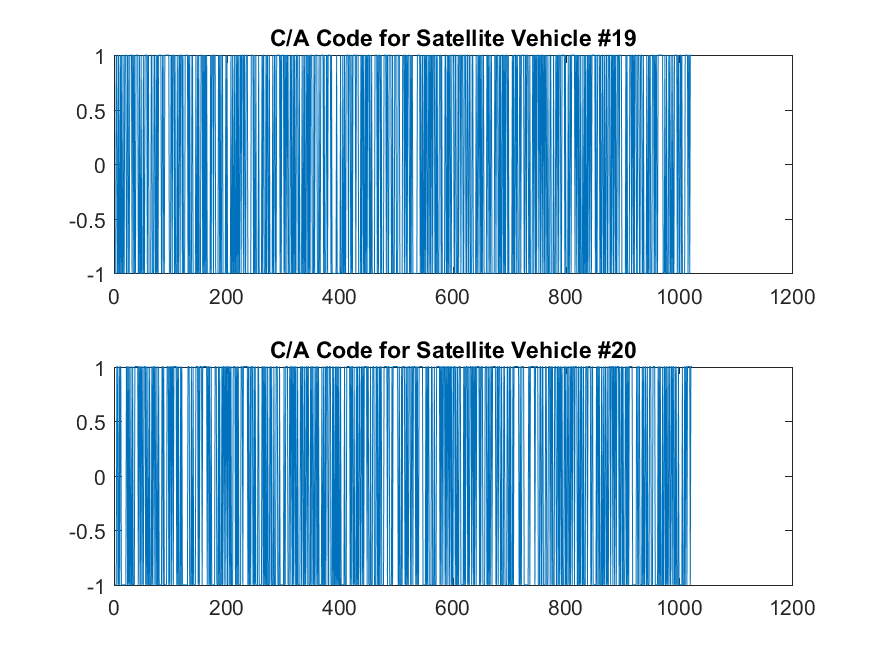
\includegraphics[width=0.8\textwidth]{HW4/latex/figures/HW4P2a.png}
    \caption{C/A Codes generated with CAcodegen.m}
    \label{fig:HW4P2a}
\end{figure*}

\item[(b)] Implement the auto-correlation function of one of the codes, for instance  \verb|ca_code|, using $1)$ linear correlation and $2)$ circular correlation. Interpret the results.

\answer{Linear correlation is performed using the built-in matlab xcorr function. The following code represents a function xcorr\_circ which performs circular correlation:}

\begin{lstlisting}[language=Matlab,numbers=left,stepnumber=1,=\scriptsize,keywordstyle=\color{blue}, commentstyle=\color{green},frame=single]
function [cxcor, lags] = xcorr_circ(a,b)

% Normalize
a = a(:) / norm(a);
b = b(:) / norm(b);

cxcor = zeros(1,length(b));
% Shift and compute cross correlation at each shift
for k=1:length(b)
    
    cxcor(k) = a' * b;
    b = circshift(b,1,1);

end
lags = [0:length(b)-1];
\end{lstlisting}


\answer{As shown in Figure \ref{fig:HW4P2b}, the result of both linear and circular autocorrelation is a single peak located at zero lag, with negligible values elswhere. This is consistent with our expectation that the codes should be poorly correlated with themselves at all but nonzero time offsets.}

\begin{figure*}[ht]
    \centering
    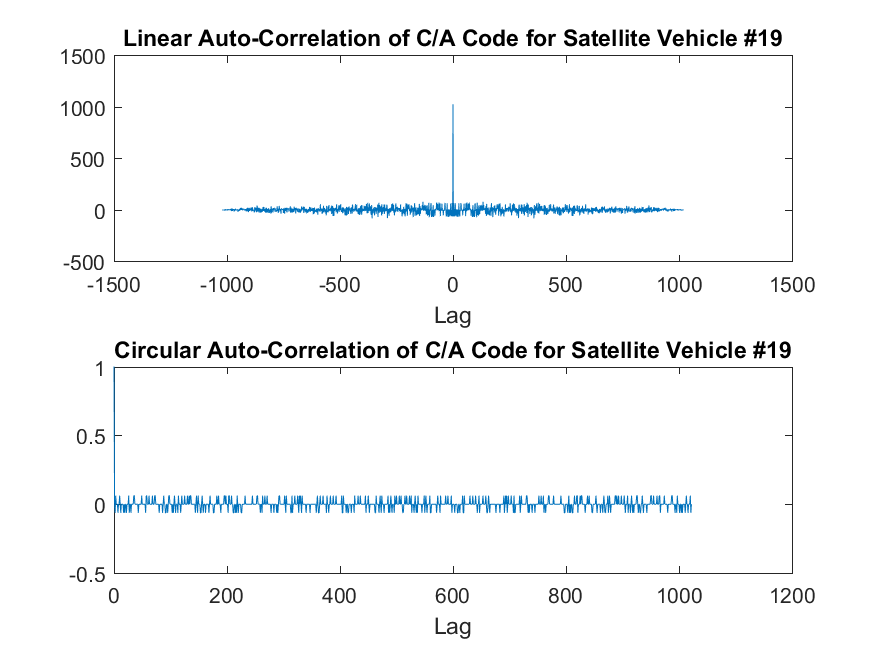
\includegraphics[width=0.8\textwidth]{HW4/latex/figures/HW4P2b.png}
    \caption{Autocorrelation of C/A Codes generated with CAcodegen.m}
    \label{fig:HW4P2b}
\end{figure*}

\item[(c)] Compute the auto-correlation of the concatenation of three PRN codes \verb|[ca_code ca_code ca_code]| with the local replica of one code \verb|ca_code|. Comment the results.


\answer{As shown in Figure \ref{fig:HW4P2c}, the result of linear cross-correlation of the C/A code with itself replicated and concatenated thrice is a peak at zero lag, and peaks at multiples of the length of the sequence, in this case -1024 and -2048. This is consistent with our expectation. Since the code repeats itself at these locations, we expect that there will be a high value where the codes align properly in the same way they do at zero lag.}


\begin{figure*}[ht]
    \centering
    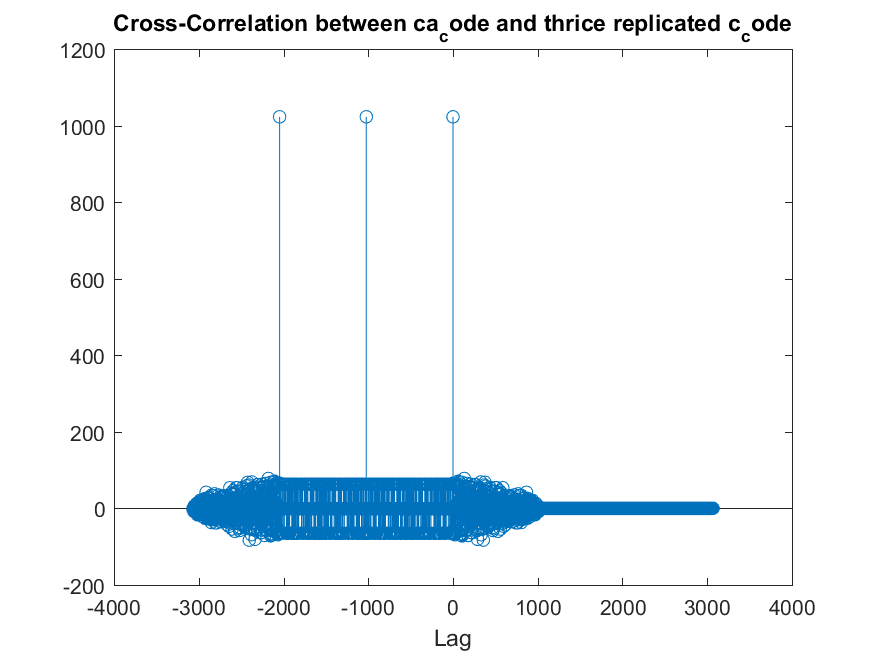
\includegraphics[width=0.8\textwidth]{HW4/latex/figures/HW4P2c.png}
    \caption{Cross-Correlation of a C/A Code with a thrice-replicated version of itself}
    \label{fig:HW4P2c}
\end{figure*}

\item[(d)] Verify the auto-correlation properties for one of the codes you generated, for instance \verb|ca_code|. Use linear and circular correlation, as in (b). Explain the results.

\answer{As previously described in part (b), Figure \ref{fig:HW4P2b} shows that the result of both linear and circular autocorrelation is a single peak located at zero lag, with negligible values elswhere. This is consistent with the property of these codes being uncorrelated with themselves at non-zero lag values, and thus we consider the auto-correlation properties to be satisfied.}

\item[(e)] Verify the cross-correlation properties between \verb|ca_code| and \verb|ca_code2|, the codes you generated. Use linear and circular correlation, as in (b). Explain your results.

\answer{As shown in Figure \ref{fig:HW4P2d}, the result of both linear and circular cross-correlation of the C/A code for Satellite Vehicle #19 with that for Sattelite Vehicle #20 is low (relative to the length of the sequence) for all lag values. Thus, we consider the property that the codes must be orthogonal to be verified.}

\begin{figure*}[ht]
    \centering
    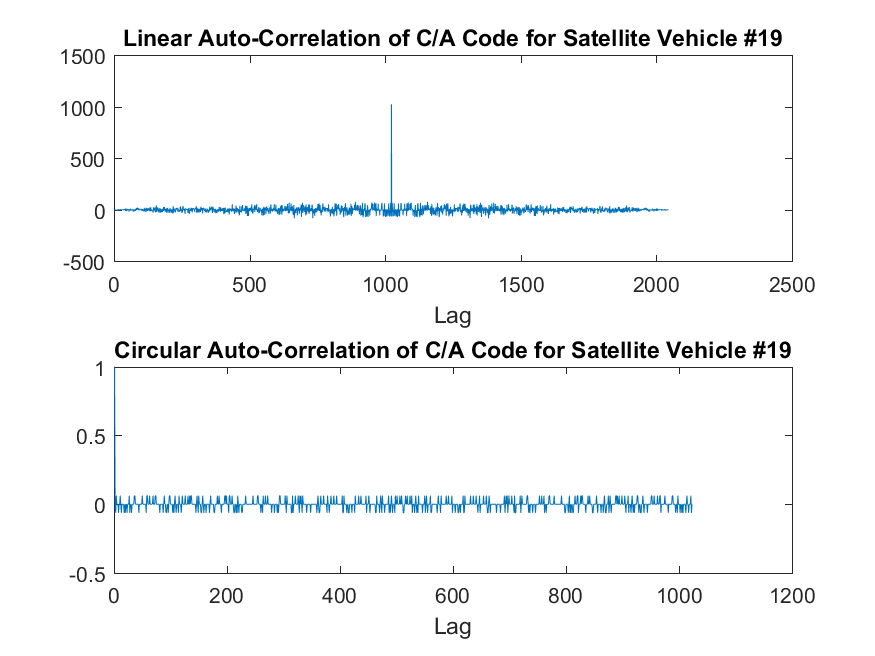
\includegraphics[width=0.8\textwidth]{HW4/latex/figures/HW4P2d.png}
    \caption{Cross-Correlation of a C/A Code with a thrice-replicated version of itself}
    \label{fig:HW4P2d}
\end{figure*}

\end{enumerate}

\pagebreak

\textbf{Problem 3}:
Load \verb|HW4P3.mat| by typing \verb|load HW4P3| in Matlab shell. That file contains a variable \verb|ca_code_hidden|, a Gold code sequence from the GPS L1 C/A constellation. Determine which satellite's code corresponds to by looping over all possible values (i.e., $32$, which is the maximum number of GPS satellites). Explain your answer.

\answer{The following code, HW4P3.m computes the correlation between the C/A codes for each of the satellites with the hidden code provided.}

\begin{lstlisting}[language=Matlab,numbers=left,stepnumber=1,=\scriptsize,keywordstyle=\color{blue}, commentstyle=\color{green},frame=single]
clearvars
close all
clc

% Load hidden code
load('HW4P3.mat');
[~,len1] = size(ca_code_hidden);

% % Load all codes
% load('Cacodes.mat');

% Generate codes
ca_code_matrix = CAcodegen([1:32]);

[nc,len2] = size(ca_code_matrix);

xcor_mat = zeros(nc,len1+len2-1);
for i = 1:size(ca_code_matrix,1)
    xcor_mat(i,:) = xcorr(ca_code_hidden, ca_code_matrix(i,:));
end

% Find maximum
[~,sat] = max(max(xcor_mat,[],2));

% Plot cross correlations
fig1 = figure;
surf(xcor_mat)
title(sprintf('Hidden code cross correlation with known C/A Codes, Max=Sat#%d',sat))
xlabel('Lag'); ylabel('Sattelite Vehicle');
zlabel('Cross Correlation');
saveas(fig1,['.\latex\figures\HW4P3.png'])
\end{lstlisting}

\answer{Figure \ref{fig:HW4P3} shows the computed cross-correlation functions. A peak can be seen at a certain lag value for Satellite Vehicle #28, which indicates that the hidden code corresponds to that for Sattelite Vehicle #28.}

\begin{figure*}[ht]
    \centering
    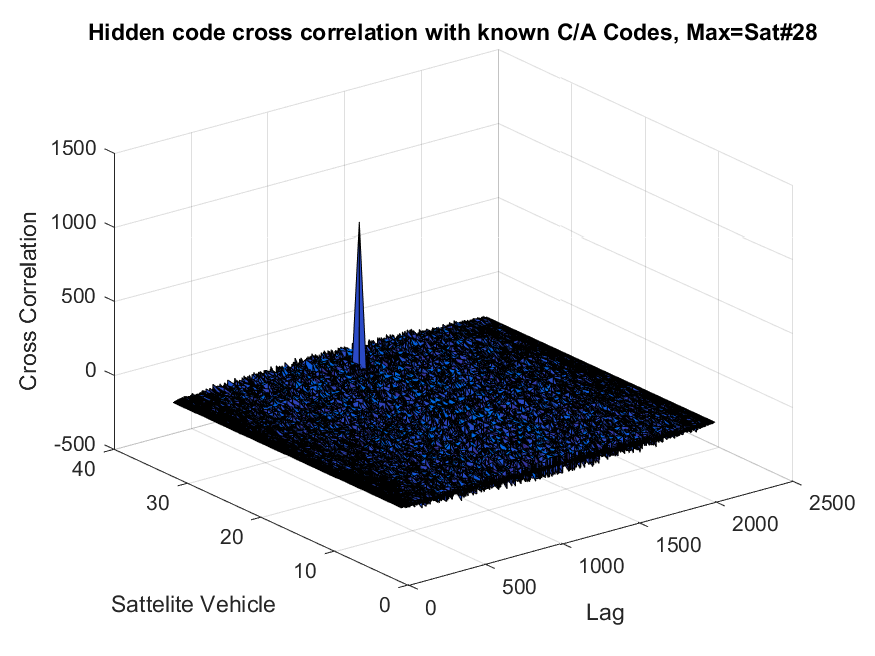
\includegraphics[width=0.8\textwidth]{HW4/latex/figures/HW4P3.png}
    \caption{Cross-Correlation of a C/A Code with a thrice-replicated version of itself}
    \label{fig:HW4P3}
\end{figure*}

\pagebreak

\textbf{Problem 4}:
Detect satellites from a real data recording. We will use a similar procedure as in Problem 3 (i.e., looping over possible satellites and correlating with the corresponding spreading code). 

Below there is a code implementing non-coherent acquisitions over \verb|Nnci| CAFs. Copy-paste this code into a script and place the file \verb|realGPSL1capture.bin| in the same folder, that file contains a real data recording of L1 band signal ($f_s=10$ MHz). You need also \verb|computeCAF.m| and \verb|ResampleCode.m| in the folder.

% \begin{lstlisting}[language=Matlab,basicstyle=\scriptsize,keywordstyle=\color{blue}, commentstyle=\color{green},frame=single]
% % signal parameters
% fs = 10e6;          % Sampling frequency
% fIF = 0;            % Intermediate frequency
% fc = 1.023e6;       % Code rate of the code [Hz]
% Tcoh = 0.001;       % Coherent integration time [s]
% Nc = Tcoh * fs;     % number of samples contained in the coherent integration time
% 
% % Acquisition parameters
% Nd = 81;            % Number of Doppler bins
% DopStep = 125;      % Doppler bin size in Hz
% secondOfData = 0.1; % Seconds of data to read
% Nnci = 1;           % number of non-coherent integrations of the CAF
% SVIDs = 1:32;          % satellite vehicles (SV) to detect [7 16 19 21 22 25]
% 
% % read file with the IF capture
% fid = fopen ('realGPSL1capture.bin','r');
% [data, cnt_data] = fread(fid, 2 * secondOfData * fs, 'int8');
% data = data(1:2:end) + 1i * data(2:2:end);
% 
% CAF_aux = zeros(Nd,Nc);
% DopplerEst = -ones(1,32);
% DelayEst = -ones(1,32);
% 
% % generate local replica and resample from Tc to Ts>Tc
% 
% % loop over all possible satellites
% for svnum = SVIDs
% 
%     [ca_code]=CAcodegen(svnum);
%     % Resample the code at data sampling frequency
%     ca_code_resampled = ResampleCode( ca_code, Nc, fs, 0, fc );   
%     
%     CAF = 0;        % initialized CAF to zero every time
%     
%     % loop to average over noncoherent integrations
%     for ii = 1:Nnci
%         y =  data( (ii - 1) * Nc + (1:Nc) ).';   % use just 1 period of code at the time
%         
%         % loop over frequency bins
%         for ff=1:Nd
%             fdbin = fIF/fs + (ff - ceil(Nd/2))*DopStep/fs;   % normalized Doppler bin
%             CAF_aux(ff,:) = computeCAF(y, ca_code_resampled, fdbin);
%         end
%         % integrate non-coherently the ii test statistics |CAF|^2 
%         CAF = CAF + abs(CAF_aux).^2;
% 
%         % plot 2D grid search
%         CAF_normalized = CAF/max(max(CAF));     % normalize to 1 the maximum value
%         
%         figure(svnum)
%         surf((0:(Nc - 1)) / fs, ((1:Nd) - ceil(Nd/2))*DopStep, CAF_normalized, 'EdgeColor', 'none');
%         axis tight, set( gca, 'FontSize', 16 )
%         xlabel('Code delay [s]'), ylabel('Doppler [Hz]')
%         title(['SV ' num2str(svnum) ' , ' num2str(ii) ' non-coherent integrations'])
% %         pause
%     end
%     pause
%     
%     % estimate Doppler (if satellite detected)
%     [~, DopInd] = max(max(CAF.'));
%     DopplerEst(svnum) = fIF + (DopInd - ceil(Nd/2))*DopStep;
% 
%     % estimate time-delay (if satellite detected)
%     [~, codInd] = max(max(CAF));
%     DelayEst(svnum) =  (codInd - 1) / fs;
% 
% end
% \end{lstlisting}

% Notice that you would need to generate the codes with \verb|CAcodegen.m|. If you were not able to work that function out, you might load \verb|CAcodes.mat|, which contains a matrix with the Gold code of each satellite (total $32$) in the corresponding row (that is, use \verb|[ca_code]=ca_code_matrix(svnum,:);| instead).


\begin{enumerate}
\item[(a)] Go through the code and explain (preferably supporting your discussion with math) the different steps implemented.

\answer{ See HW4P4.m. For a given satellite, the algorithm performs the following steps:

\begin{enu}
\item[(i)] Resample the code by replicating the points in the C/A code in order to create a sequence of chips with length defined by the coherent integration time. The number of replications needed to form a chip with the correct sample rate is given by the ratio of the sample rate to the chipping rate, $f_s/f_c$. The elements of the code are replicated to form these chips, and the entire code is replicated in order to form a sequence which spans the entire integration time.

\item[(ii)] A sequence of data of length defined by the non-coherent integration time is "recorded" and used the resampled code is used to compute the cross ambiguity function for a set of doppler frequencies on either side of the intermediate frequency.

\item[(iii)] The cross ambiguity functions computed for each non-coherent integration period are added together to form the approximation of the cross ambiguity function for the entire integration duration.

\end{enu}

}

\item[(b)] Run the code with \verb|Nnci=1|. Explain the processing that takes place in the receiver in this configuration. How many satellites are you able to clearly detect (i.e., distinguish from noise floor)?

\answer{Visual inspection reveals that, with the possible exception of Satellite Vehicle \#7, no clear peaks are distinguishable from the noise floor for any satellites. Plots are not included space.}

\item[(c)] Gradually increase \verb|Nnci| from $1$ to $10$ non-coherent integrations. Explain the processing that takes place in the receiver in this configuration. How many satellites are you able to clearly detect (i.e., distinguish from noise floor)? Explain the results.

\answer{Attempting to identify satellite detection through visual inspection, increasing the number of non-coherent integrations to 4 additionally reveals clear peaks for Satellite Vehicle \#25, \#22, \#19, and \#16 in addition to \#7. This is due to the fact that averaging over a longer duration reduces the impact of the uncorrelated noise within the cross ambiguity function, allowing the signal to be more visible.

Increasing the number of non-coherent integrations all the way to 10 does not reveal any more satellites, most likely because there are none. Although increasing the number of integrations makes detection easier, there is nothing more to be gained by increasing the duration once all of the satellites that are present have been detected.}

\item[(d)] At the light of the results, which satellites are more likely to be present in the capture? Once a satellite is acquired, which information is passed on to the tracking loops?

\answer{The satellites which are more likely to be present in the capture are those which exhibit the greatest signal to noise ratio within the cross ambiguity function. Based on our inspection for this data those are Satellite Vehicle \#25, \#22, \#19, \#16 and \#7. Following this step of the reciever, the cross ambiguity function as well as estimates of the doppler shift and time-delay for each of the detected satellites would be relayed to the tracking portion of the receiver.}

\end{enumerate}


\end{document}




